\documentclass[a4paper]{article}
\usepackage[a4paper,top=2cm,bottom=2.5cm,left=1.5cm,right=1.5cm,marginparwidth=1.75cm]{geometry}

%% Language and font encodings
\usepackage[english]{babel}
\usepackage[utf8x]{inputenc}
\usepackage{listings}
\usepackage{helvet}

%% Sets page size and margins
\usepackage{float}

%% Useful packages
\usepackage{amsmath}
\usepackage[colorinlistoftodos]{todonotes}
\usepackage[colorlinks=true, allcolors=blue]{hyperref}
\usepackage{listings}
\usepackage{graphicx}
\graphicspath{ {./images/} }
% \DeclareGraphicsExtensions{.pdf,.jpg,.png}

%% defined colors
\definecolor{Blue}{rgb}{0,0,0.5}
\definecolor{Green}{rgb}{0,0.75,0.0}
\definecolor{LightGray}{rgb}{0.6,0.6,0.6}
\definecolor{DarkGray}{rgb}{0.3,0.3,0.3}

%% Packages added by me
\usepackage{url}
\usepackage{hyperref}
\usepackage{quoting}
\usepackage[font={small,it}]{caption}
\usepackage{subcaption}

\graphicspath{{./images/}}

\title{Assignment: Applied Data Science Capstone project}
\author{Marc Jellema} \date{\today}

\begin{document}
\maketitle

\abstract{
This report is a deliverable for my capstone project \textit{Battle of the neighbourhoods}, part of my graduation for my \textbf{IBM Data Science Professional certificate}. The assignment was to define a challenge that was to be solved by using the FourSquare API. Nowadays almost anything you need can be found online, including public data sets to use freely. I tapped into the public domain data sets with key figures from the Netherlands. Combining the FourSquare with the Dutch key figures showed a strong correlation between house prices and the number of restaurants in the neighbourhood. Before this correlation is to be used in other algorithms, I strongly advice to use more detailed data sets to underwrite the conclusion found during my assignment. Feel free to send me an email on {\href{mailto:mjellema@omnia.nl}{mjellema@omnia.nl}} if you like to discuss this report in more detail.

% TODO abstract needs to hold the executive summary as well

\section*{Introduction}
I tasked myself with the assignment to find additional ways to enhance automatic estimation of house prices in the Netherlands. The use of the \textbf{FourSquare} API is mandatory for this assignment, part of the IBM Data Science professional certificate \cite{IBM1}. As a tech savvy person myself, I'd heard of FourSquare and I do remember seeing the FourSquare logo on venues in the past, but never came across its footprint in the Netherlands. Wondering if I could use the FourSquare API in finding an answer for a challenge in the Netherlands, I did some research and as it turns out, the FourSquare database is more than comprehensive enough to use for data science challenges in the Netherlands as well. Not knowing a single person actively using FourSquare to let their friends know where they check-in, it puzzled me how FourSquare actually accumulates their data. James D. Walsh wrote a nice article \cite{FS1} on how FourSquare accomplishes this. Enough about FourSquare for now, let's focus on introducing the question I want to answer with help of the FourSquare API and the data it can provide:
\medskip
\begin{quote}
\textit{Based on \textbf{FourSquare} data, can we find a correlation between the average house price, the number of restaurants and the number of inhabitants in the provinces of the Netherlands?}
\end{quote}
\medskip
Although the COVID pandemie is having an impact on the overall economy world wide, it seems house prices have not yet taken a hit due to the pandemic. Startups like \textbf{Promodomo} \cite{Promo} use algorithms to calculate house prices, even when they are not on the market yet. Algorithms like Promodomo's always benefit from additional sources to enrich their calculation. Searching for a correlation based on FourSquare data is just one off the many possibilities to augment the estimation of house prices and this is why I choose to take this challenge and come up with answers in this capstone project of my IBM Data Science Professional certificate. 
\section{Data}
To answer the challenge I needed the following data points:
\medskip
\begin{enumerate}
  \item Number of inhabitants per province in the Netherlands
  \item Average house price per province in the Netherlands
  \item Number of restaurants per province in the Netherlands
\end{enumerate}
\medskip
Ad 1. The number of inhabitants per province in the Netherlands can be downloaded from the Centraal Bureau voor Statistiek \textbf{(CBS)}: a government owned, freely accessible web site with tons of statistical datasets (over 4K of them!) to use in all kind of analysis. I did some research on which table would best provide my need for the number of inhabitants per province and its title turns out to be \texttt{[Regionale kerncijfers Nederland]}. The resulting data frame, including some data cleaning done like removing substring \texttt{[(PV)]} from the province name, is in figure \ref{inhabitant}.  
\\\\
Ad 2. The average house price per province in the Netherlands in 2019 also can be downloaded from the CBS, this time based on the table with title \texttt{[Bestaande koopwoningen; gemiddelde verkoopprijzen, regio]}. After a bit of cleaning and tweaking (i.e. 'Friesland' ≠ 'Fryslân' and some column renaming had to be adjusted to make the dataset comprehensible for our international readers) the resulting data frame is in figure \ref{avgprice}.
\\\\
Ad 3. The third dataset, the number of restaurants, came from FourSquare. I needed to find all restaurants within each province of the Netherlands. The FourSquare API has the following two drawbacks that I needed to overcome: the non commercial API limits the returned number of venues per call to max 100 and although the results have a \texttt{[state]} field, the API doesn't allow searching per state. The limit of max 100 venues per call I overcame with the help of the material I found of a fellow course student Guillermo (G.) Bareirro \cite{STUDENT1}. FourSquare returns max 100 venues per call, but if you make the call specific enough, the total results will not grow above the limit. Using the categories listed bij G. Bareirro, I was able to split querying all restaurants into their separate categories and thereafter grouped and summed them with pandas standard data frame functionality. To overcome the second drawback of not being able to query FourSquare by state and knowing that an estimate of the restaurants per province would be sufficient for my analyses, I queried the restaurants (via their respective subcategories) in the capital city of each province. For the province of Noord-Holland I made an exception: the capital of Noord-Holland is Haarlem, but Amsterdam (the capital of the Netherlands) is by far a more important city in the province of Noord-Holland so I took the liberty of using Amsterdam instead of Haarlem as the anchor point for the FourSquare queries. The data frame is in figure \ref{restaurants}.
\\\\
The three data frames used in the analyses for this assignment are in the images below:
\medskip
\begin{figure}[H]
	\begin{subfigure}{0.33\textwidth}
		\centering
		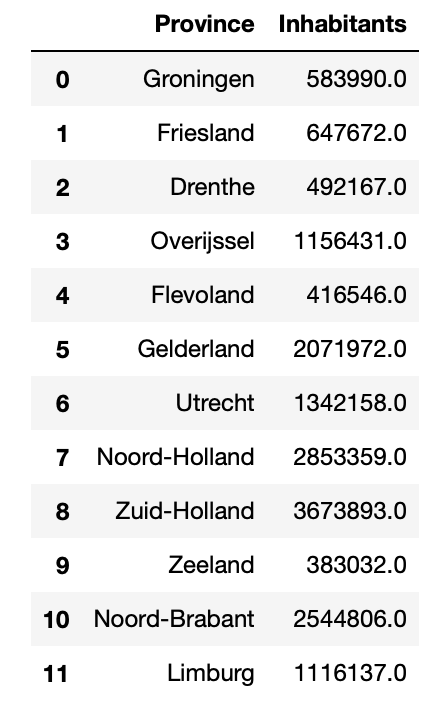
\includegraphics[scale=.4]{Inhabitants.png} 
		\caption{Inhabitants from StatLine \cite{CBS1}}
		\label{inhabitant}
	\end{subfigure}
	\begin{subfigure}{0.33\textwidth} 
		\centering 
		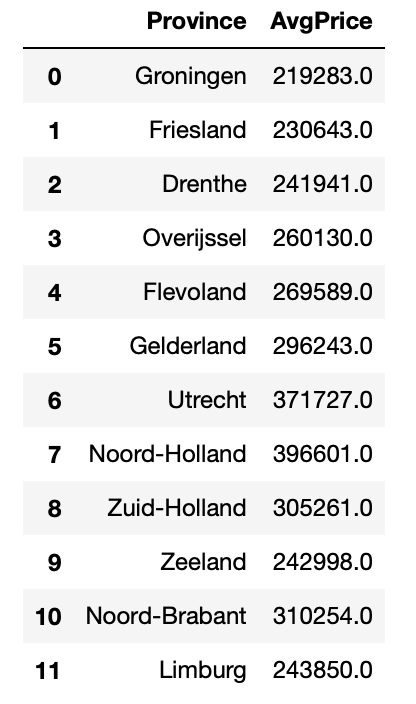
\includegraphics[scale=.4]{AvgPrice.png} 
		\caption{Average Price from StatLine \cite{CBS2}}
		\label{avgprice}
	\end{subfigure}
	\begin{subfigure}{0.33\textwidth}
		\centering
		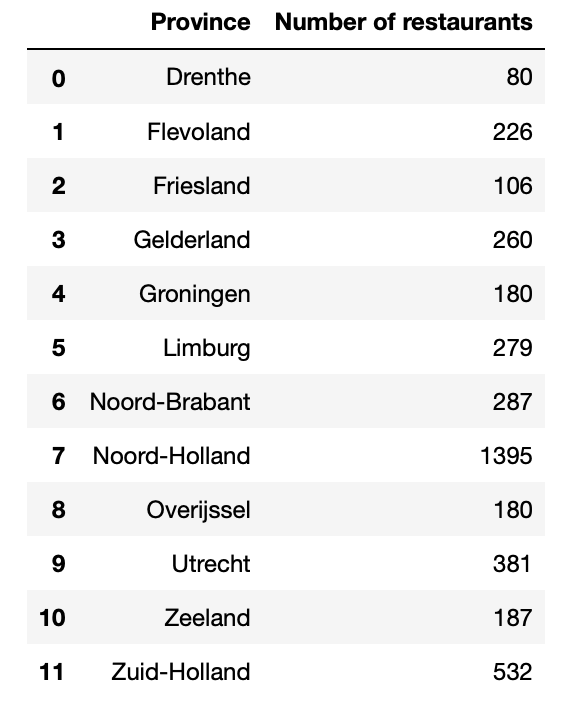
\includegraphics[scale=.4]{Restaurants.png} 
		\caption{Restaurants from FourSquare \cite{FS2}}
		\label{restaurants}
	\end{subfigure}
\caption{Cleaned data frames as used in analysis}
\end{figure}
\medskip
After submitting this data section for the first part of my graduation I came across a dataset that turned out to be very helpful in showing the final results on a map of the Netherlands and it was too compelling for me to leave this opportunity out of this report. So the fourth part added to the data frames was a \textbf{GeoPandas} data frame with the geometries of each province in the Netherlands. Thanks to the excellent blog post of Artem (A.) Zapara \cite{STUDENT2} I was able to get the final bit of information I needed and added it to the resulting data frame of figure \ref{resultset}.
\medskip
\begin{figure}[H]
	\center
	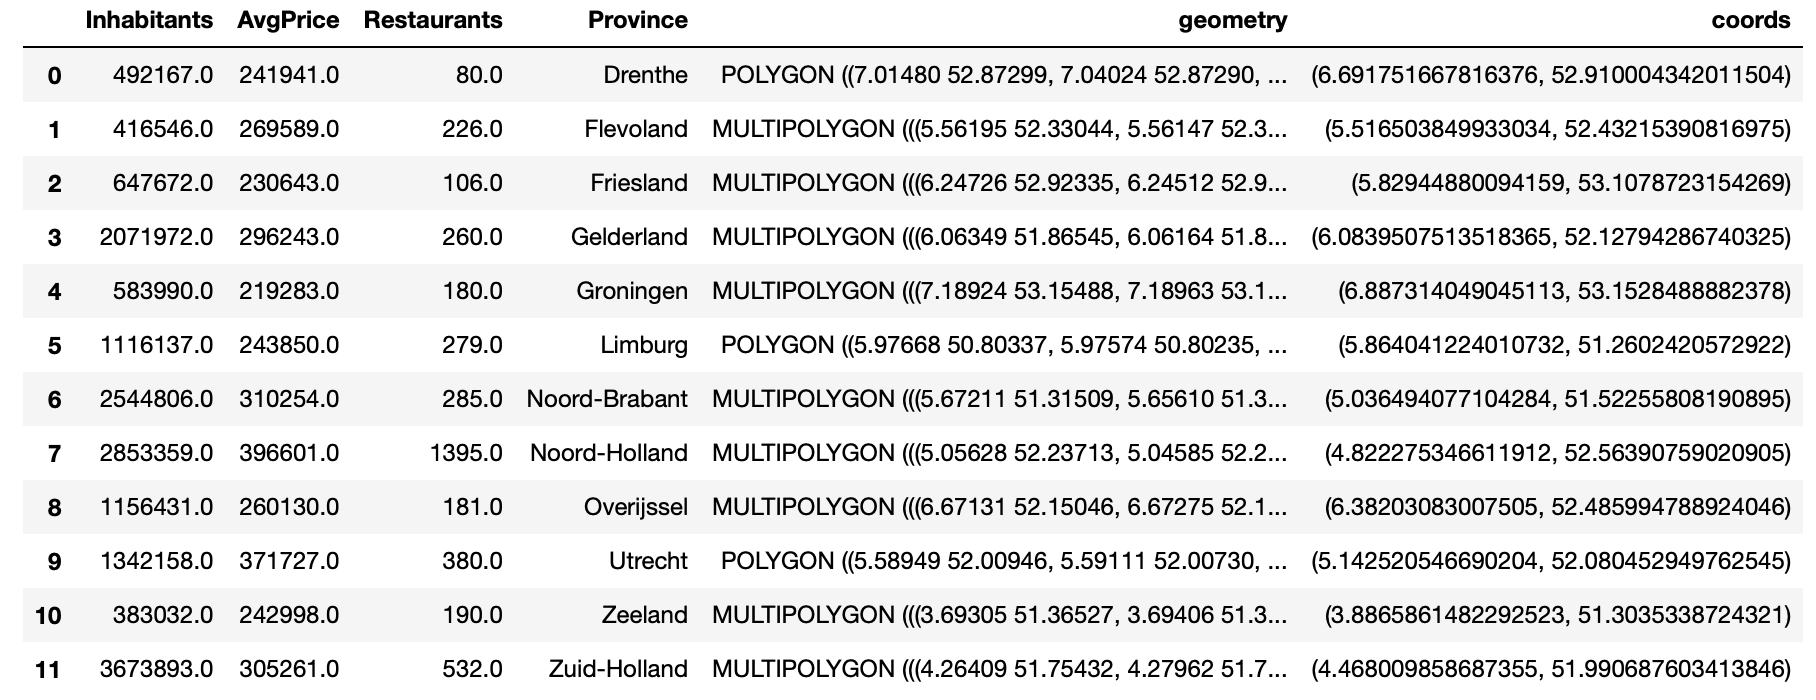
\includegraphics[scale=.4]{ResultSet.png}	
	\caption{Result set for analyses and reporting}
	\label{resultset}
\end{figure}
\medskip
As always I was very impressed with the work of fellow programmers / students: almost any programming question already has been answered (although sometimes in parts) and can be found on Google. If you know the right keywords and have enough time to keep searching, you will find most of the puzzle pieces readably available. You just need to connect the dots so to say. On top of that, Python keeps amazing me for the strength of its coding syntax: import the right libraries and with just a couple of lines of code you can generate, filter and merge data frames into a data frame ready for takeoff.



\section{Methodology \& Analyses}
Next to the data and the master data frame I explained in the previous data section, for this assignment I used a public GitHub repository \cite{GIT1} to store my documentation, images, notebook and report connected to this assignment. Everything was developed and programmed locally on my Macbook pro in a Python 3 / Anaconda setup and committed to the repository with the GitHub desktop client for OSX \cite{GIT2}. I used the regular Python libraries used in many data science assignments like \texttt{[pandas]} for handling data frames and \texttt{[requests]} for handling data retrieval via URL requests. For charting and graphics I used a combination of the \texttt{[matplotlib]} and \texttt{[seaborn]} libraries.
\\\\
Finding correlations can be easy if you have the master data frame well prepared. The \texttt{[analyses data frame]} as shown in the data section (see figure \ref{resultset}) only uses one line of code to come up with the correlation matrix. Both the input (\texttt{analyses data frame}) and the output (\texttt{correlation matrix}) are in the images below:
\\
\medskip
\begin{figure}[H]
	\begin{subfigure}{0.5\textwidth}
		\centering
		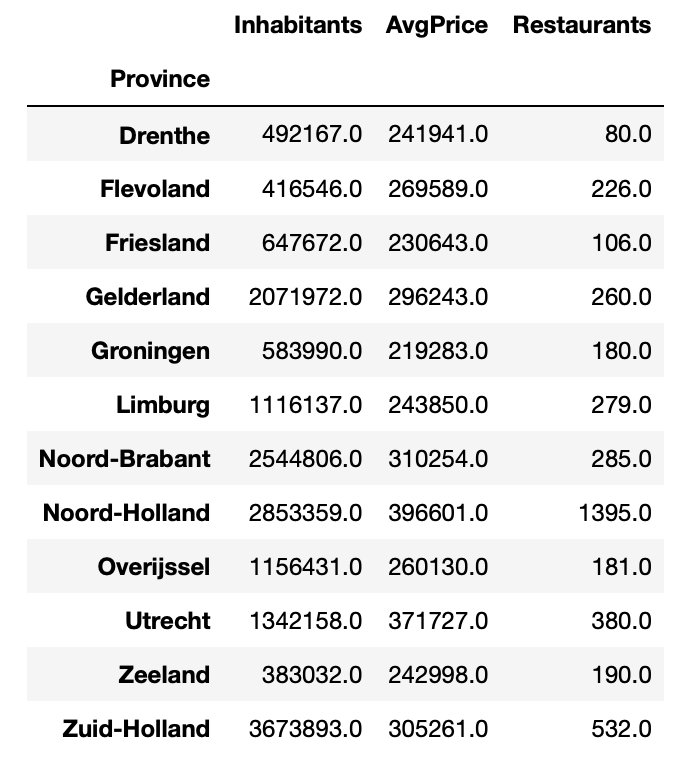
\includegraphics[scale=.4]{AnalysesSet} 
		\caption{}
	\end{subfigure}
	\begin{subfigure}{0.5\textwidth}
		\centering
		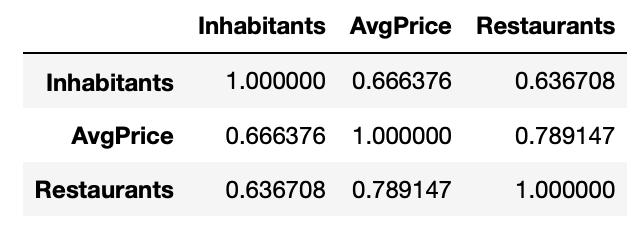
\includegraphics[scale=.4]{CorrMatrix}
		\caption{}
		\label{corMatrix}
	\end{subfigure}
\caption{Analysis data frame and calculates correlation matrix}
\end{figure}
\medskip
Based on the calculated correlation coefficients, I was able to do the analysis and come up with the desired results, which I compared to the rule of thumb mentioned on ResearchGate \cite{ART1} about the value of correlation coefficients. The IBM Data Science Professional course on Coursera covers a lot of model training and learning modules and during the course I had plenty of opportunity to play around with most modern types of analysis and machine learning techniques. The question underlying this report however, doesn't need a lot of computer calculation power to solve. Basically the methodology followed to answer the challenge summarises as follows:
\medskip
\begin{enumerate}
	\item Get the venues data from FourSquare
	\item Get the demographic data from CBS
	\item Get the price data from CBS
	\item Get the geo data from Arcgis
	\item Combine \& clean the data into a result set
	\item Use default routines of Pandas to calculate the correlation coefficients
	\item Analyse the results
	\item Plot the results on a map of the Netherlands
\end{enumerate}
\medskip

\section{Results}
\section{Discussion}
Looking back on the results, one could say that statistically the answers found on the two questions hold, but of course there is a lot to say about the depth of this analysis and if the results are generally applicable in the real world. For example, let's look at the level of detail of the data sets used in the analysis. The data frames used are condensed data sets. Look at the data set with the average house price: this set holds the average price based on thousands of transactions. For more in depth analyses and better understanding of the results, it might be better to use the underlying data set of all these transactions and not the condensed average. The same holds for the set of restaurants. The correlation is now based on the number of restaurants in the main or capital city of a province. Taking just the restaurants of the focal point of the province was done due to the limitations of the free requests possible to FourSquare. If we would use a data set with all venues instead of just a this subset, the correlation could turn out differently. Last but not least, just looking at restaurants being listed in FourSquare, without examining the venues in more detail like looking at reviews and actual use (=number of guests per annum) of these venues, there is a lot of room for improvement on the thoroughness of the analysis.
\section{Conclusion}
To summarise, with the data sets I used, I've been able to give a statistical answer on both of the questions raised but before the results can safely augment an automatic house estimation algorithm, more work has to be done.
\section{Acknowledgements}
I would like to take the opportunity to thank Guido van Rossum: the creator of Python. I've been programming since ANSI C was the standard and Turbo Pascal 5.0 was the new kid on the block, but in all those years I never came across a language that uses soo few lines of code to accomplish so much. As mentioned before, adding just a few libraries and you have a very powerful programming toolbox at hand.
\\\\
Next to Guido, I'd like to thank all the programmers and contributors that share their code, their examples and answer the questions raised by co-programmers on platforms like Stack Overflow, Medium, GitHub and many others: without your explanations my life as a python programmer would have been a lot tougher.
\\\\
Let me sign off with thanking IBM and Coursera for setting up this course. I was a bit reluctant at first having to complete nine courses to get a single certificate and that much of the reviewing and grading would be done by co students, but you guys have managed to setup an honourable community and the course materials where tough enough to make me proud that I have passed the test.

\bibliographystyle{ieeetr}
\bibliography{bibfile}

\end{document}